\documentclass{beamer}
\let\vec\mathbf
\mode<presentation>
\usepackage{amsmath}
\usepackage{amssymb}
%\usepackage{advdate}
\usepackage{adjustbox}
%\usepackage{subcaption}
\usepackage{enumitem}
\usepackage{multicol}
\usepackage{mathtools}
\usepackage{listings}
\usepackage{url}
\usetheme{Boadilla}
\usecolortheme{lily}
\setbeamertemplate{footline}
{
  \leavevmode%
  \hbox{%
  \begin{beamercolorbox}[wd=\paperwidth,ht=2.25ex,dp=1ex,right]{author in head/foot}%
    \insertframenumber{} / \inserttotalframenumber\hspace*{2ex} 
  \end{beamercolorbox}}%
  \vskip0pt%
}
\setbeamertemplate{navigation symbols}{}
\providecommand{\nCr}[2]{\,^{#1}C_{#2}} % nCr
\providecommand{\nPr}[2]{\,^{#1}P_{#2}} % nPr
\providecommand{\mbf}{\mathbf}
\providecommand{\pr}[1]{\ensuremath{\Pr\left(#1\right)}}
\providecommand{\qfunc}[1]{\ensuremath{Q\left(#1\right)}}
\providecommand{\sbrak}[1]{\ensuremath{{}\left[#1\right]}}
\providecommand{\lsbrak}[1]{\ensuremath{{}\left[#1\right.}}
\providecommand{\rsbrak}[1]{\ensuremath{{}\left.#1\right]}}
\providecommand{\brak}[1]{\ensuremath{\left(#1\right)}}
\providecommand{\lbrak}[1]{\ensuremath{\left(#1\right.}}
\providecommand{\rbrak}[1]{\ensuremath{\left.#1\right)}}
\providecommand{\cbrak}[1]{\ensuremath{\left\{#1\right\}}}
\providecommand{\lcbrak}[1]{\ensuremath{\left\{#1\right.}}
\providecommand{\rcbrak}[1]{\ensuremath{\left.#1\right\}}}
\theoremstyle{remark}
\newtheorem{rem}{Remark}
\newcommand{\sgn}{\mathop{\mathrm{sgn}}}

\providecommand{\res}[1]{\Res\displaylimits_{#1}} 
\providecommand{\norm}[1]{\left\lVert#1\right\rVert}
\providecommand{\mtx}[1]{\mathbf{#1}}

\providecommand{\fourier}{\overset{\mathcal{F}}{ \rightleftharpoons}}
%\providecommand{\hilbert}{\overset{\mathcal{H}}{ \rightleftharpoons}}
\providecommand{\system}{\overset{\mathcal{H}}{ \longleftrightarrow}}
	%\newcommand{\solution}[2]{\textbf{Solution:}{#1}}
%\newcommand{\solution}{\noindent \textbf{Solution: }}align
\providecommand{\dec}[2]{\ensuremath{\overset{#1}{\underset{#2}{\gtrless}}}}
\newcommand{\myvec}[1]{\ensuremath{\begin{pmatrix}#1\end{pmatrix}}}

\title{Matrices in Geometry - 1.9.6}
\author{EE25BTECH11017 Mahesh Chollangi}
\date{Sept, 2025}

\begin{document}

\maketitle


\section{Problem}
\begin{frame}
\frametitle{Problem Statement}
 If $\vec{Q}\brak{0,1}$ is equidistant from $\vec{P}\brak{5,-3}$ and $\vec{R}\brak{x,6}$, find the value of x.
\end{frame}

\section{Solution}
\begin{frame}{Solution}
   \textbf{Given: } 
$\vec{Q}\myvec{0\\1}$, $\vec{P}\myvec{5\\-3}$ and a point $\vec{R} \myvec{x \\ 6}$ such that $\vec{Q}$ is equidistant from $\vec{P}$ and $\vec{R}$. 
\begin{align}
     \therefore \norm{\vec{Q}-\vec{P}}=\norm{\vec{Q}-\vec{R}}\\
    \text{On squaring both the sides, we get }\\
    \norm{\vec{Q}-\vec{P}}^2=\norm{\vec{Q}-\vec{R}}^2\\
    \myvec{\vec{Q}-\vec{P}}^{\top}\myvec{\vec{Q}-\vec{P}}=\myvec{\vec{Q}-\vec{R}}^{\top}\myvec{\vec{Q}-\vec{R}}
\end{align}
\end{frame}

\begin{frame}{Solution}
\begin{align}
    \vec{Q}^{\top}\vec{Q} - 2\vec{Q}^{\top}\vec{P} + \vec{P}^{\top}\vec{P} =\vec{Q}^{\top}\vec{Q} - 2\vec{Q}^{\top}\vec{R} + \vec{R}^{\top}\vec{R}\\
    \norm{\vec{P}}^2 - \norm{\vec{R}}^2=2\vec{Q}^{\top}\myvec{\vec{P}-\vec{R}}\\
    \norm{\myvec{5\\-3}}^2 - \norm{\myvec{x\\6}}^2=2\myvec{0 & 1}\myvec{5-x \\ -9}\\
    25+9- x^2 -36=2\brak{0 + (-9)}\\
    -2 -x^2=2\brak{-9} \implies x^2=16 \implies x= -4 , x= 4
\end{align}
\end{frame}



\section{Final Answer}
\begin{frame}{Final Answer}
\begin{align}
    \text{Hence, the final answer is }\fbox{x= -4, x= 4} 
\end{align}
\begin{figure}
    \centering
    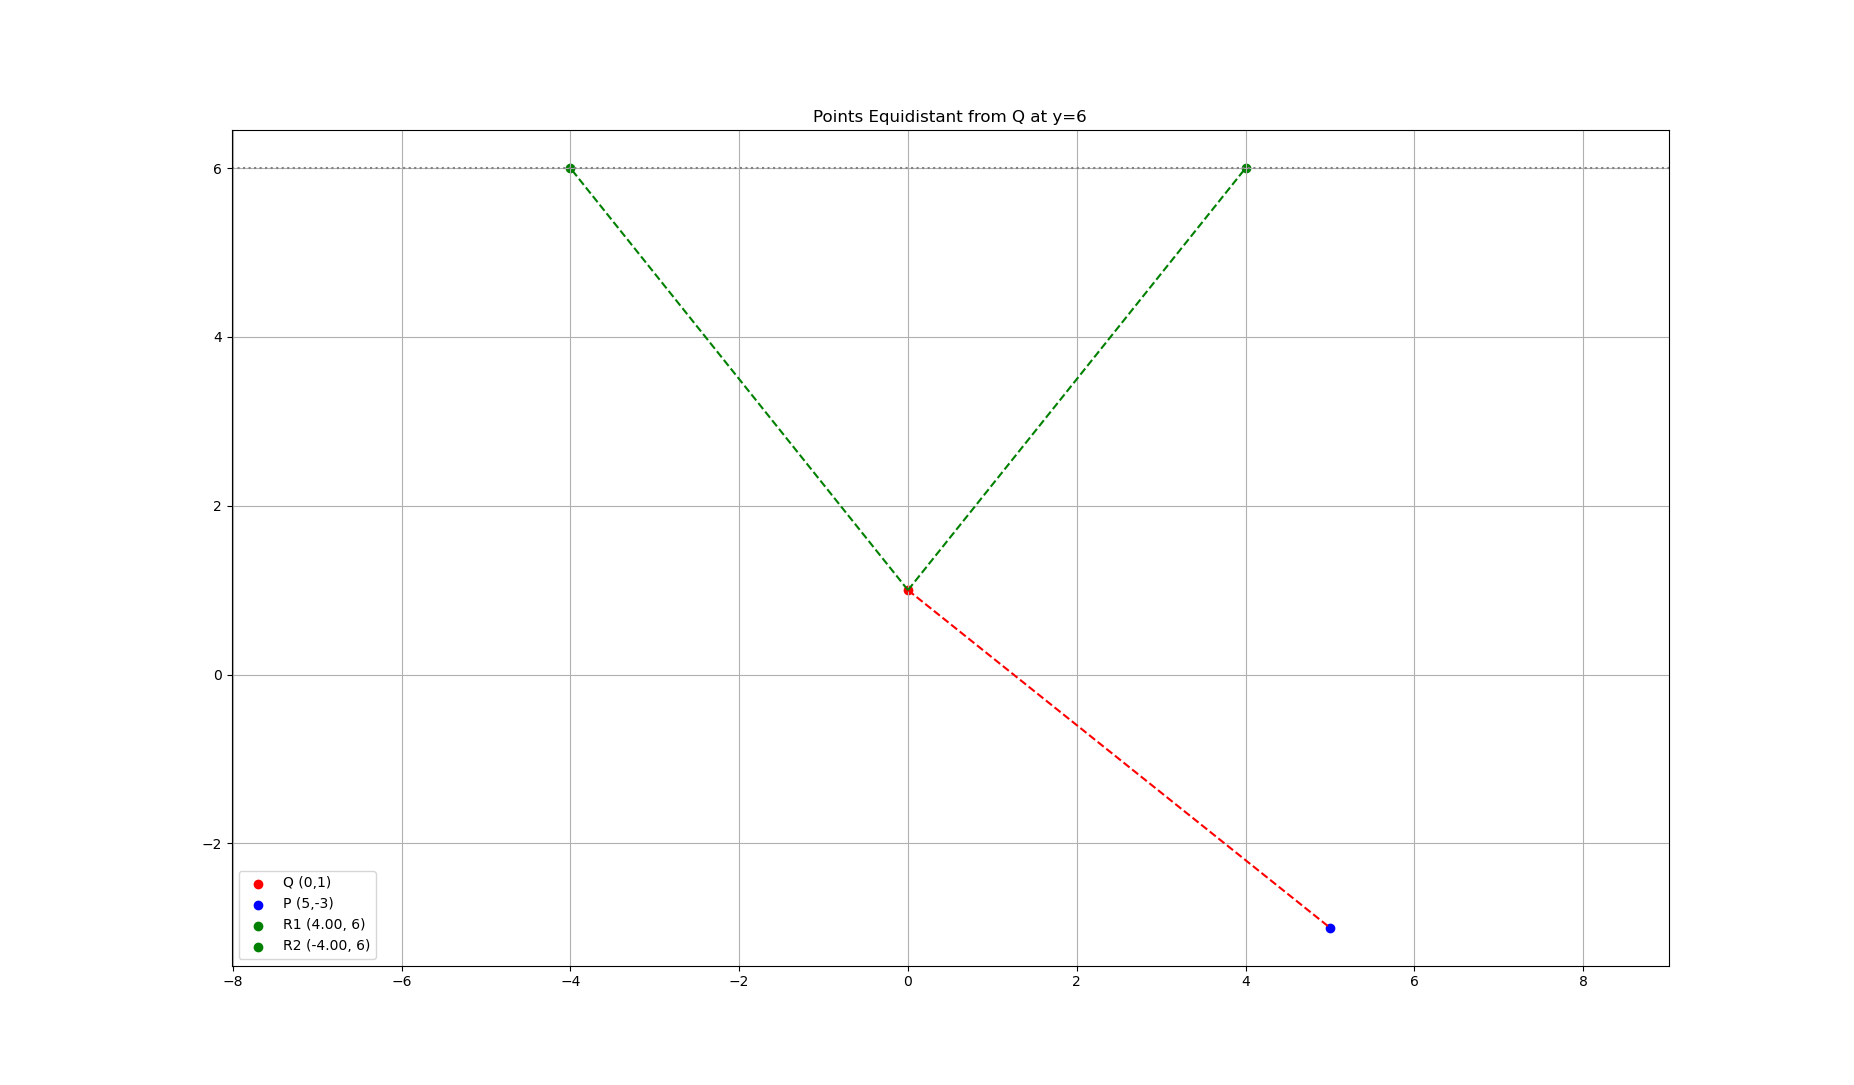
\includegraphics[width=1\columnwidth]{Figs/Figure_1.png}
\end{figure}
\end{frame}

\begin{frame}[fragile]
    \frametitle{C Code - Function to Find distance between points}

    \begin{lstlisting}
    #include <math.h>

// Array to store roots
static float roots[2];

// Function to return pointer to roots array
float* get_roots() {
    // distance between Q(0,1) and P(5,-3)
    float d1 = sqrt((5-0)*(5-0) + (-3-1)*(-3-1)); // sqrt(41)
    
    // Solve for x: x^2 + 25 = d1^2 -> x^2 = 16
    roots[0] = 4.0;
    roots[1] = -4.0;
    
    return roots;
}
\end{lstlisting}

\end{frame}

    \begin{frame}[fragile]
    \frametitle{Python Code - for plotting}
    \begin{lstlisting}
    import matplotlib.pyplot as plt
import numpy as np

# Fixed points Q and P
Q = np.array([0, 1])
P = np.array([5, -3])

# Calculate distance between Q and P
d = np.linalg.norm(P - Q)

# y-coordinate of R
y_R = 6

\end{lstlisting}
\end{frame}

 \begin{frame}[fragile]
    \frametitle{Python Code - for plotting}
    \begin{lstlisting}
# Find x-coordinates of points R on line y=6 such
that distance(Q, R) = distance(Q, P)
x_R1 = np.sqrt(d**2 - 25)
x_R2 = -x_R1

R1 = np.array([x_R1, y_R])
R2 = np.array([x_R2, y_R])

# Plot points
plt.scatter(*Q,color='red',label='Q (0,1)')
plt.scatter(*P,color='blue',label='P (5,-3)')
plt.scatter(*R1,color='green',label=f'R1({x_R1:.2f},6)')
plt.scatter(*R2,color='green',label=f'R2({x_R2:.2f},6)')

\end{lstlisting}
\end{frame}

\begin{frame}[fragile]
    \frametitle{Python Code - for plotting}
    \begin{lstlisting}
# Plot lines from Q to P and Q to R points
plt.plot([Q[0], P[0]], [Q[1], P[1]], 'r--')
plt.plot([Q[0], R1[0]], [Q[1], R1[1]], 'g--')
plt.plot([Q[0], R2[0]], [Q[1], R2[1]], 'g--')

plt.axhline(y=y_R, color='gray', linestyle=':')

plt.legend()
plt.title('Points Equidistant from Q at y=6')
plt.grid(True)
plt.axis('equal')
plt.show()

\end{lstlisting}
\end{frame}

\end{document}